%%%%%%%%%%%%%%%%%%%%%%%%%%%%%%%%%%%%%%%%%%%%%%%%%%%%%%%%%%%%%%%%%%%
%% This document is part of the set of template files
%% for the uwyo_thesis style. This is your main file that
%% helps compile the entire document; each individual chapter
%% should be a separate file that is brought in using the
%% "\include{}" commands shown below.
%%
%% Step one: rename this file to something specific to you, such as
%% "Smith_thesis.tex" so your eventaul PDF file will end up having the
%% name "Smith_thesis.pdf."  You can also rename any individual chapter
%% files; if you do, be sure to make the appropriate change to the
%% "\include{}" commands below.
%%
%% Important: only *this* file should be compiled by LaTeX.
%% The individual chapter files are *not* standalone files.
%%
%% For interdisciplinary programs such as Neuroscience, see the
%% special section below
%%%%%%%%%%%%%%%%%%%%%%%%%%%%%%%%%%%%%%%%%%%%%%%%%%%%%%%%%%%%%%%%%%%

%%%%%%%%%%%%%%%%%%%%%%%%%%%%%%%%%%%%%%%%%%%%%%
%\documentclass[12pt,oneside,openany]{book}  % single-sided printing
\documentclass[12pt]{book}                  % double-sided printing
%% First line above assumes single-sided printing.
%% For double-sided (duplex) printing use the second line instead.
%% The duplex printing version is best for your final version of the document
%%%%%%%%%%%%%%%%%%%%%%%%%%%%%%%%%%%%%%%%%%%%%%
\usepackage{uwyo_thesis} % the main style file
%%% Many common packages are already loaded by the style file
%%% Add any others below
%\usepackage{??}


%%% Note about your title:
%%% Due to limitations in the UW Banner system, you may want to limit your
%%% thesis/dissertation titles to the following:
%%%  Masters thesis titles:  214 characters including spaces
%%%  Ph.D. dissertation titles: 208 characters including spaces



%%%%%%%%%%%%%%%%%%%%%%%%%%%%%%%%%%%%%%%%%%%%%%%%%%%
%%% set these values for your particular document and
%%% uncomment the lines below as needed
%%%%%%%%%%%%%%%%%%%%%%%%%%%%%%%%%%%%%%%%%%%%%%%%%%%
\mastersthesis % uncomment this if a Masters thesis; comment out if PhD
%\thesisdraft  % uncomment to put time/date/draft stamp in header
%\renewcommand{\thesisauthorLname}{your last name}
%\renewcommand{\thesisauthorFMname}{your first name and middle initial}
%\renewcommand{\thesismonth}{your graduation month}
%\renewcommand{\thesisyear}{your graduation year}
%\renewcommand{\thesisDefenseDate}{the exact day you defend your thesis}
%%% NOTE: you must enter the same title for both \thesistitle and \abstitle below
% Do not use all upper case! That will be done for you where needed.
%\renewcommand{\thesistitle}{your document title}
%\renewcommand{\abstitle}{\ul{your document title}}
% Must be exactly the same as \thesistitle
%\renewcommand{\thesisDeptName}{your academic department or interdisciplnary program}
%\renewcommand{\thesisDeptHead}{name of your academic department head or program chair}
%\renewcommand{\thesisCollegeName}{your college}
%\renewcommand{\thesisDeanName}{name of your college Dean}
%\renewcommand{\thesisDegreeArea}{what your degree is in}
%\renewcommand{\thesisauthorpreviousdegrees}{any of your previous degrees}
%\renewcommand{\lstlistlistingname}{my program listings} % if you want an alternate name for the list
%\renewcommand{\thesisDeptHeadTitle}{Interim Head} % if you're between Dept Heads
%\renewcommand{\thesisDeanTitle}{Interim Dean} % if you're between Deans

%\renewcommand{\thesisdedication}{your dedication} % no length limit, but don't get carried away!

%%%%%%%% Interdisciplinary programs section %%%%%%%%%%%%%%%%%%%
%% You need to define things a bit differently:
%% \renewcommand{\thesisDeptName}{the name of your interdisciplnary program}
%% \renewcommand{\thesisDeptHead}{name of your interdisciplinary program chair}
%% \renewcommand{\thesisDeptHeadTitle}{Program Chair}
%% \renewcommand{\thesisCollegeName}{University of Wyoming}
%% \renewcommand{\thesisDeanName}{name of the UW Provost}
%% \renewcommand{\thesisDeanTitle}{Provost}
%%%%%%%%%%%%%%%%%%%%%%%%%%%%%%%%%%%%%%%%%%%%%%%%%%%%%%%%%%%%%%%


%%% Required: insert your committee member names inside the curly braces
%%% then uncomment the needed lines
% \thesisCommitteeChair{}  % this is your advisor
% \thesisFirstMember{}  % this should be the member *outside* your department
% \thesisSecondMember{}
% \thesisThirdMember{}
% \thesisFourthMember{}
% \thesisFifthMember{}
% \thesisSixthMember{}
% \thesisExternalMember{Carol Danvers}  % a member from another university, not normally used
% only uncomment the line below if you actually have an external member
% \thesisExternalTitle{External Member}  % Not normally used


%%%%%%%%%%%%%%%%%%%%%%%%%%%%%%%%%%%
\begin{document}

% Print initial frontmatter

%%%%%%%%%%%%%%%%%%%%%%%%%%%%%%%%%%%%%%%%%%%%%
%%% Generate the committee page.
%%%  If you want to save a page, you can comment
%%%  this out for early drafts as it isn't needed
%%%  until you're ready for the final version.
\thesisCommitteePage
%%%

%%% the abstract page
\begin{thesisabstract}
This is where you write your abstract.  Here are the guidelines on
the abstract according to UW and the
ProQuest/UMI organization (the company that archives theses and dissertations from
universities worldwide).


For a masters thesis, the abstract should ideally be around 60 to 80
words in length.  If you must, you can exceed this length, but the
abstract cannot exceed one page.  Any abstract text that exceeds
150 words will be truncated to the first 150 words (and any non-textual content will
be removed) by ProQuest for the online databases, although your full abstract will
be preserved in the complete electronic (PDF) version of your thesis.


For a Ph.D.\ dissertation, the abstract should ideally be no longer than 350 words. If
the abstract exceeds 350 words, it will be truncated to the first 350 words (and any
non-textual content will be removed) by ProQuest for the online databases, although your
full abstract will be preserved in the electronic (PDF) version of your dissertation. In
any case, the dissertation abstract cannot exceed two pages (one page is preferred).

New paragraph. This line is meant to check the margins and text
appearance. This line is meant to check the margins and text
appearance. This line is meant to check the margins and text
appearance. This line is meant to check the margins and text
appearance. This line is meant to check the margins and text
appearance. This line is meant to check the margins and text
appearance. This line is meant to check the margins and text
appearance.

New paragraph. This line is meant to check the margins and text
appearance. This line is meant to check the margins and text
appearance. This line is meant to check the margins and text
appearance. This line is meant to check the margins and text
appearance. This line is meant to check the margins and text
appearance. This line is meant to check the margins and text
appearance. This line is meant to check the margins and text
appearance.

New paragraph. This line is meant to check the margins and text
appearance. This line is meant to check the margins and text
appearance. This line is meant to check the margins and text
appearance. This line is meant to check the margins and text
appearance. This line is meant to check the margins and text
appearance. This line is meant to check the margins and text
appearance. This line is meant to check the margins and text
appearance.



\end{thesisabstract}

 \thesistitlepage        % print title page
 \thesiscopyrightpage    % print the copyright page
 % comment out line below to eliminate the optional dedication page, if you really can't think of anyone!
 \thesisdedicationpage   % print the dedication page

% Generate and print the lists
 \tableofcontents        % table of contents
 \listoffigures          % List of Figures
 \listoftables           % List of Tables
 % comment out line below if you have no program listings!!!
 \mylistoflistings      % List of program listings


%% acknowledgments section: don't forget to thank your committee
%% members, any funding sources/grants, even your Mom and Dad if you want
\begin{thesisacknowledgments}
This is where you write any paragraphs you want to show up on the Acknowledgments page.
Traditionally, you use this space to thank your committee members for their help, any
funding sources such as an NSF grant that helped you, and so on.  This section is up to
you (no page or word limit, but exercise restraint) as long as it is written in a
professional manner. Be careful you don't end up with a messy page break, such as when
the automatic insertion of your name, the university name, and the month and date at the
end of this environment is the only thing that shows up on the next page.  Write more or
less text here to fix it!

New paragraph. This line is meant to check the margins and text appearance. This line is
meant to check the margins and text appearance. This line is meant to check the margins
and text appearance. This line is meant to check the margins and text appearance. This
line is meant to check the margins and text appearance. This line is meant to check the
margins and text appearance. This line is meant to check the margins and text appearance.

\end{thesisacknowledgments}


%%%%%%%%%%%%%%%%%%%%%%%%%%%%%%%%%%%%%%%%%%%%%%%%%%%%
%%% Now this is where your various chapters come in
%%%%%%%%%%%%%%%%%%%%%%%%%%%%%%%%%%%%%%%%%%%%%%%%%%%%

%% Abbreviations is an optional entry, placed either at the front or at the end of the document
%% Uncomment the line below if you want abbreviations to be part of the front matter, before Chapter 1
%%%%%%%%%%%%%%%%%%%%%%%%%%%%%%%%%%%%%%%%%%%%%%%%%%%%%%%%%%%%%%%%%%%%%%%%%%%%%
%% This file can be used to generate a list of symbols, abbreviations, etc.
%% as part of the front matter, BEFORE Chapter 1.
%%   For use with theses or dissertations using uwyo_thesis.sty
%%
%%   Version: 1.00
%%   Last modified: 26 August 2019
%%
%%%%%%%%%%%%%%%%%%%%%%%%%%%%%%%%%%%%%%%%%%%%%%%%%%%%%%%%%%%%%%%%%%%%%%%%%%%%%


%%%%%%%%%%%%%%%%%%%%%%%%
\chapter*{Abbreviations, Acronyms, and Symbols}
\label{Abbreviations}  % for you to be able to refer to this appendix in the main text
\addcontentsline{toc}{chapter}{Abbreviations, Acronyms, and Symbols} % make this show up in TOC


% % % % % % % % % % % % % % % % % % % % % % % % % % % % %
{ % begin special environment for abbreviations  -- modify only with great care!

 \setlength{\parindent}{0pt}

%%%%% commands just for this file %%%%%%%%%%%%%%%%%%%%%%%
 \newcommand{\abbrltr}[1]{% command for letter section
   \bigskip
   \framebox{\textbf{#1}}
   \medskip
 }
 \newlength{\abbrwidth}
 \newlength{\abbrdef}
 \setlength{\abbrwidth}{0.6in}  % adjust for longest abbreviation
 \setlength{\abbrdef}{\textwidth}
 \addtolength{\abbrdef}{-\abbrwidth}
 \newcommand{\abbr}[2]{% command for an entry
   \begin{tabular}{p{\abbrwidth}p{\abbrdef}}
     \textbf{#1} & {#2}
   \end{tabular}

 }

%%%%%%%%%%%%%%%%%%%%%%%%%%%%%%%%%%%%%%%%%%%%%%%%%%%%%%%%%
%%%%%%%%%%%%%%%%%%%%%%%%
%% start appendix text %%
%%%%%%%%%%%%%%%%%%%%%%%%

This is a partial list of abbreviations, acronyms, and symbols used in the
text, provided in the hope that it will be helpful to some readers.

\abbrltr{Symbols}

\abbr{$(\:)$}{used for a continuous function.}

\abbr{$[\:\:]$}{used for a discrete function.}

\abbrltr{Greek Letters}

\abbr{$\alpha$}{feedback coefficient for simple IIR filters, such as those used for a
type of echo generation for guitar special effects.}

\abbr{$\lambda$}{wavelength.}

\abbr{$\pi$}{ratio of a circle circumference to diameter,
3.1415926535897932\ldots}

\abbr{$\tau$}{time constant.}

\abbr{$\omega$}{radian frequency.}

\abbrltr{A}

\abbr{$a$}{filter coefficient associated with an output term, $y$.
When used in a transfer function, the $a$ coefficients are
associated with the denominator of the transfer function.}

\abbr{$A$}{vector or array containing all of the $a$ terms.}


\abbr{ADC}{analog-to-digital converter.}

\abbr{AIC}{analog interface circuit (see codec).}

\abbr{AGC}{automatic gain control.}

\abbr{AM}{amplitude modulation.}

\abbr{ARM}{Advanced RISC Machine, a 32-bit reduced instruction set computer (RISC)
instruction set architecture (ISA) developed by ARM Holdings.}

\abbr{AWGN}{additive white Gaussian noise.}


\abbrltr{B}

\abbr{$b$}{filter coefficient associated with an input term, $x$.
When used in a transfer function, the $b$ coefficients are
associated with the numerator of the transfer function.}

\abbr{$B$}{vector or array containing all of the $b$ terms.}

\abbr{$BW$}{bandwidth of a bandpass signal.}

\abbr{BP}{bandpass.}

\abbr{BPF}{bandpass filter.}

\abbr{BPSK}{binary phase shift keying.}

\abbrltr{C}

\abbr{C}{value of capacitance.}

\abbr{CD-ROM}{Compact disk read-only memory.}

\abbr{CISC}{complex instruction set computer.}

\abbr{codec}{coder-decoder.  An integrated circuit that contains
both an ADC and a DAC.}

\abbr{CPU}{central processing unit.}

\abbrltr{D}

\abbr{DAC}{digital-to-analog converter.}

\abbr{D.C.}{direct current (0 Hz).}

\abbr{DDS}{direct digital synthesizer or direct digital
synthesis.}

\abbr{DF-I}{direct form I.}

\abbr{DF-II}{direct form II.}

\abbr{DFT}{discrete Fourier transform.}

\abbr{DMA}{direct memory access.}

\abbr{DSK}{DSP starter kit.}

\abbr{DSP}{digital signal processing or digital signal processor.}

\abbr{DTFT}{discrete-time Fourier transform.}

\abbr{DTMF}{dual-tone, multiple-frequency signals as defined by telephone companies.}

\abbrltr{E}

\abbr{EDMA}{enhanced direct memory access.}

\abbrltr{F}

\abbr{FCC}{Federal Communications Commission.}

\abbr{FIR}{finite impulse response.}

\abbr{FFT}{fast Fourier transform.}

\abbr{FT}{Fourier transform.}

\abbr{$\mathcal{F}$}{Fourier transform.}

\abbr{$\mathcal{F}^{-1}$}{inverse Fourier transform.}

\abbr{$f_h$}{highest or maximum frequency that is present in a
signal.}

\abbr{$F_s$}{sample frequency (samples/second) = $1/T_s$.}

\abbrltr{G}

\abbr{GPP}{general purpose processor.}

\abbr{GPU}{graphics processing unit.}

\abbrltr{H}

\abbr{$H(e^{j\omega})$}{discrete-time frequency response.}

\abbr{$H(j\omega)$}{continuous-time frequency response.}

\abbr{$h[n]$}{discrete-time impulse response or unit sample
response.}

\abbr{$h[t]$}{continuous-time impulse response.}

\abbr{$H(s)$}{continuous-time transfer or system function.}

\abbr{$H(z)$}{discrete-time transfer or system function.}

\abbr{HDTV}{high-definition television.}

\abbr{HP}{highpass.}

\abbr{HPF}{highpass filter.}

\abbr{HPI}{host port interface.}

\abbr{Hz}{hertz (cycles per second).}

\abbrltr{I}

\abbr{IF}{intermediate frequency.}

\abbr{IFFT}{inverse fast Fourier transform.}

\abbr{IIR}{infinite impulse response.}

\abbr{ISA}{instruction set architecture.}

\abbr{ISR}{interrupt service routine.}

\abbrltr{J}

\abbr{$j$}{$\sqrt{-1}$; identifies the imaginary part of a complex number. Some authors
use $i$ instead of $j$.}

\abbr{JTAG}{Joint Test Action Group, commonly used as the name of a debugging interface
for printed circuit boards and IC chips. Formalized as IEEE Std 1149.1 in 1990.}

%\abbrltr{K}

%\abbr{$k$}{dummy index of summation used in the convolution sum.}

\abbrltr{L}

\abbr{$\mathcal{L}$}{Laplace transform.}

\abbr{$\mathcal{L}^{-1}$}{inverse Laplace transform.}

\abbr{L}{value of inductance.}

\abbr{LFSR}{linear feedback shift register.}

\abbr{LP}{lowpass.}

\abbr{LPF}{lowpass filter.}

\abbr{LSB}{lower sideband, also used for least significant bit.}


\abbrltr{M}

\abbr{M}{the number of bands in a graphic equalizer.}

\abbr{MA}{moving average.}

\abbr{McASP}{multi-channel audio serial port.}

\abbr{McBSP}{multi-channel buffer serial port.}

\abbr{ML}{maximum likelihood.}

\abbrltr{N}

\abbr{$n$}{index or sample number.}

\abbr{$N$}{often used as filter order; in other contexts, it is used for the length of a
sequence, or for the length of an FFT.}

\abbr{NCO}{numerically controlled oscillator.}


\abbrltr{O}

\abbr{OMAP}{Open Multimedia Application Platform, a family of proprietary multi-core
system on chips (SoCs) by Texas Instruments.}


\abbrltr{P}

\abbr{PC}{personal computer.}

\abbr{PCM}{pulse code modulation.}

\abbr{PLL}{phase-locked loop.}

\abbr{PN}{pseudonoise.}

\abbr{PSK}{phase shift keying.}


\abbrltr{Q}

\abbr{$Q$}{quality factor.  $Q$ = bandwidth of a BP filter divided
by its center frequency.  The higher the value of $Q$, the more
selective the BP filter is.}

\abbr{QAM}{quadrature amplitude modulation.}

\abbr{QPSK}{quadrature phase shift keying.}

\abbrltr{R}

\abbr{$r$}{magnitude of a pole.  This is a measure of how far the
pole is from the origin.}

\abbr{R}{value of resistance.}

\abbr{RC}{resistor-capacitor.}

\abbr{RISC}{reduced instruction set computer.}

\abbr{RF}{radio frequency.}

\abbrltr{S}

\abbr{$s$}{the Laplace transform independent variable, $s = \sigma
+ j\omega$.}

\abbr{SoC}{system on chip.}

\abbrltr{T}

\abbr{$\tau$}{a dummy variable often used in convolution.}

\abbr{$t$}{time.}

\abbr{$T$}{period of a signal or function.}

\abbr{TED}{timing error detector.}

\abbr{$T_s$}{sample period = $1/F_s$.}

\abbr{TI}{Texas Instruments.}

\abbrltr{U}

\abbr{$u[n]$}{discrete-time unit step function.}

\abbr{$u(t)$}{unit step function.}

\abbr{U.S.}{United States (of America).}

\abbr{USB}{upper sideband; also used for Universal Serial Bus.}

\abbrltr{V}

\abbr{$V$}{voltage in Volts.}

\abbr{$V_{in}$}{input voltage.}

\abbr{$V_{out}$}{output voltage.}

\abbr{VLIW}{very long instruction word; this is a type of
architecture for DSPs.}

\abbrltr{W}

\abbr{winDSK}{original Windows-based program for the C31 DSK,
created by Mike Morrow.}

\abbr{winDSK6}{Windows-based program, the follow-on to winDSK, for the C6x DSK series. It
was created by Mike Morrow.}

\abbr{winDSK8}{Windows-based program, the follow-on to winDSK6, for the OMAP-L138
multi-core board). It was created by Mike Morrow.}

\abbrltr{X}

\abbr{$X(j\omega)$}{result of the Fourier transform
$\mathcal{F}\{x(t)\}$; it shows the frequency content of $x(t)$.}

\abbr{$x[n]$}{a discrete-time input signal.}

\abbr{$x(t)$}{a continuous-time input signal.}

%\newpage

\abbrltr{Y}

\abbr{$Y(j\omega)$}{result of the Fourier transform
$\mathcal{F}\{y(t)\}$; it shows the frequency content of $y(t)$.}

\abbr{$y[n]$}{a discrete-time output signal.}

\abbr{$y(t)$}{a continuous-time output signal.}

\abbrltr{Z}

\abbr{$z$}{the independent transform variable for discrete-time signals and systems.}

\abbr{$z^{-1}$}{a delay of 1 sample.}

\abbr{$Z_c$}{impedance of a capacitor.}

\abbr{$\mathcal{Z}$}{$z$-transform.}

\abbr{$\mathcal{Z}^{-1}$}{inverse $z$-transform.}


% % % % % % % % % % % % % % % % % % % % % % % % %
} % end environment for zero \parindent  -- do not remove this curly brace

%\mycleardoublepage

%%%%%%%%%%%%%%%%%%%%%%%%
%%% end appendix text %%%
%%%%%%%%%%%%%%%%%%%%%%%%


 % 

% Bring in the chapter files -- \input is more efficient than \include
% This file is for chapter 1

\chapter{Introduction}

\section{The Need for This Research}

There are many good reference sources to help you make the most out of using \LaTeX, both on the Internet and as books.  There is also a huge worldwide group of users who willingly share their expertise as needed.  Take a look at the web page for the \TeX\ Users Group (TUG) at \url{www.tug.org}.

A blank line starts a new paragraph. 
This is meaningless text used only to test the
margins and such. This is meaningless text used only to test the
margins and such. This is meaningless text used only to test the
margins and such. This is meaningless text used only to test the
margins and such. This is meaningless text used only to test the
margins and such. This is meaningless text used only to test the
margins and such. This is meaningless text used only to test the
margins and such.

\section{Previous Research}

This is meaningless text used only to test the margins and such.
This is meaningless text used only to test the margins and such.
This is meaningless text used only to test the margins and such.
This is meaningless text used only to test the margins and such.
This is meaningless text used only to test the margins and such.
This is meaningless text used only to test the margins and such.
This is meaningless text used only to test the margins and such.

This is meaningless text used only to test the margins and such.
This is meaningless text used only to test the margins and such.
This is meaningless text used only to test the margins and such.
This is meaningless text used only to test the margins and such.
This is meaningless text used only to test the margins and such.
This is meaningless text used only to test the margins and such.
This is meaningless text used only to test the margins and such.
This is meaningless text used only to test the margins and such.

\section{Dissertation Overview and Organization}

This is meaningless text used only to test the margins and such.
This is meaningless text used only to test the margins and such.
This is meaningless text used only to test the margins and such.
This is meaningless text used only to test the margins and such.
This is meaningless text used only to test the margins and such.
This is meaningless text used only to test the margins and such.
This is meaningless text used only to test the margins and such.
This is meaningless text used only to test the margins and such.
This is meaningless text used only to test the margins and such.
This is meaningless text used only to test the margins and such.
This is meaningless text used only to test the margins and such.
This is meaningless text used only to test the margins and such.
This is meaningless text used only to test the margins and such.
This is meaningless text used only to test the margins and such.
 % chapter 1
% This file is for chapter 2

\chapter{Theoretical Background}

\section{My First Section}

This first work theoretical in this area was performed by Golomb
\cite{Golomb82}. This is meaningless text used only to test the
margins and such. This is meaningless text used only to test the
margins and such. This is meaningless text used only to test the
margins and such.
\subsection{A Subsection}
Bringing this work to practical fruition has been attributed to
Dixon \cite{Dixon94}. This is meaningless text used only to test
the margins and such. This is meaningless text used only to test
the margins and such. This is meaningless text used only to test
the margins and such. 
\subsection{Another Subsection}
Let's try out an equation. The expression for a double-sideband
(with carrier) AM signal is
\begin{equation}
s_{\mathrm{AM}}(t)=A_c[1+m(t)]\cos(\omega_c t) \label{eq:dsb_lc}
\end{equation}
where $A_c$ is the amplitude of the carrier, $m(t)$ is the message
signal (with amplitude always $\le 1$ to prevent overmodulation),
and $\omega_c$ is the carrier frequency expressed in radians/sec
\cite{Couch01}. In order to recover the message signal from
(\ref{eq:dsb_lc}), it is necessary to extract the envelope of the
signal $A_c[1+m(t)]$. Once the envelope is obtained, the DC
component can be removed with a DC blocking filter, leaving $A_c
m(t)$, which is a scaled version of the original message signal.
This is meaningless text used only to test the margins and such.
This is meaningless text used only to test the margins and such.
This is meaningless text used only to test the margins and such.
This is meaningless text used only to test the margins and such.
This is meaningless text used only to test the margins and such.

\section{My Second Section}

Let's see how a floating figure is formatted.  As we see in
Figure~\ref{fg:ctf}, the optical measures of MTF and CTF are
not equal \cite{smith90}.
\begin{figure}
\centering
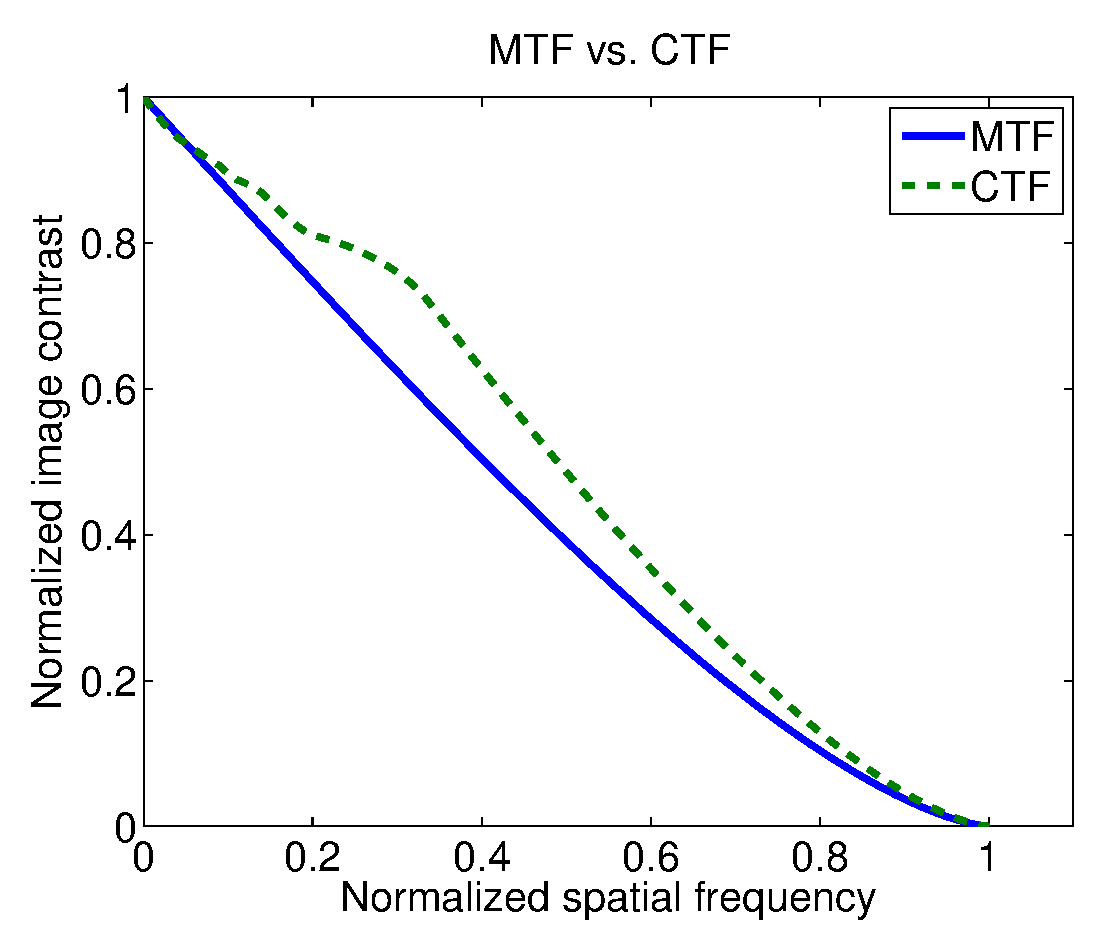
\includegraphics[width=0.7\textwidth]{ctf.eps}
\caption[MTF versus CTF.]{A comparison of the modulation transfer
function and the contrast transfer function.} \label{fg:ctf}%
\end{figure}
Note that for a figure environment, the caption comes \emph{after} the
definition of the figure itself.

Sometimes you want to combine two subfigures into one main figure.  The \pc{subfig} package, loaded automatically with the UW thesis and dissertation files, can easily do this.  You just use the \pc{\subfloat} command as shown in the \TeX\ source file below (it won't show up in the PDF file, of course, only the result of the command shows up there).

Some common shapes for individual positive and negative lenses, and their associated names, are shown in Fig.~\ref{fg:lens_types}.  
\begin{figure}%
\centering
\subfloat[Positive (converging) lenses.]{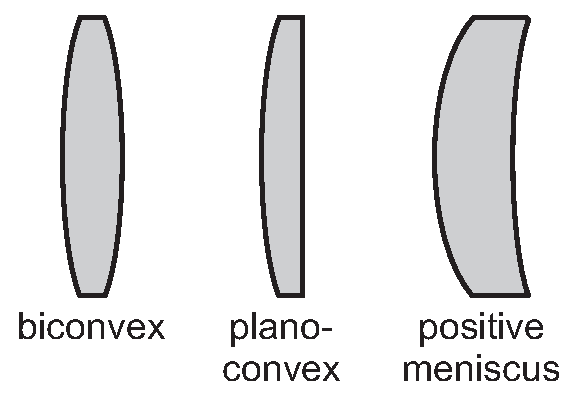
\includegraphics[width=0.35\textwidth]{lens_positive3.eps}}\qquad\qquad
\subfloat[Negative (diverging) lenses.]{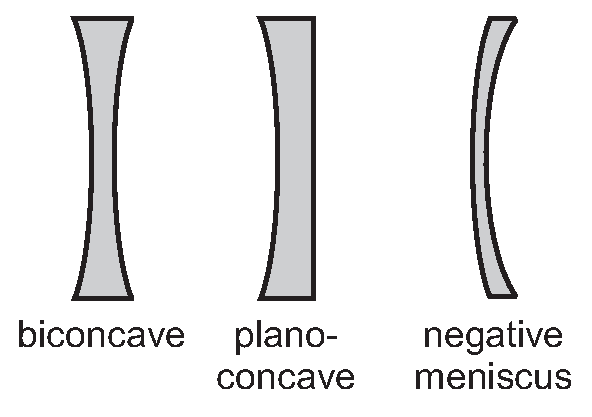
\includegraphics[width=0.35\textwidth]{lens_negative3.eps}}
\caption{Common types of lenses.}
\label{fg:lens_types}
\end{figure}

How about listings of computer programs? The main program
(\pc{main.c}) is very basic, as shown below. Note that unless your
advisor objects, program listings should be single-spaced, which
can be controlled with the \pc{\spacing} command as shown.  If you 
have longer and/or many program listings, it's usually better to 
place them in an appendix.

\begin{spacing}{1}
\begin{lstlisting}[caption={Main program for simple frame-based processing
  using ISRs.},label={cd:FrameMain_isr}]{}
#include "..\Common_Code\DSK_Config.h" 
#include "frames.h"

int main() {
    // initialize all buffers to 0
    ZeroBuffers();

    // initialize DSK for selected codec
    DSK_Init(CodecType, TimerDivider);

    // main loop here, process buffer when ready
    while(1) {
        if(IsBufferReady()) // process buffers in background
            ProcessBuffer();
    }
}
\end{lstlisting}
\end{spacing}
\noindent Wasn't that a nice program?  % see how to avoid an indented line?

How about some \ml\ code? Note you have to specify the language
since \ml\ wasn't the default language in the ``listings'' setup.

\begin{spacing}{1}
\begin{lstlisting}[language=matlab,%
caption={Simple \ml\ FIR filter example.}]{}
%  This m-file is used to convolve x[n] and B[n]
%
%  Assumes that both x[n] and B[n] start at n = 0
%
%  written by Dr. Thad B. Welch, PE {t.b.welch@ieee.org}
%  copyright 2001
%  completed on 13 December 2001 revision 1.0

% Simulation inputs
x = [1 2 3 0 1 -3 4 1];             % input vector x[n]
B = [0.25 0.25 0.25 0.25];          % FIR filter coefficients B[n]

% Calculated terms
PaddedX = [x zeros(1,length(B)-1)]; % zeros pads x[n] to flush the filter
n = 0:(length(x) + length(B) - 2);  % plotting index for the output
y = filter(B, 1, PaddedX);          % performs the convolution

% Simulation outputs
stem(n, y)                          % output plot generation
ylabel(`output values')
xlabel(`sample number')
\end{lstlisting}
\end{spacing}

New paragraph. This is meaningless text used only to test the
margins and such. This is meaningless text used only to test the
margins and such. This is meaningless text used only to test the
margins and such. This is meaningless text used only to test the
margins and such. This is meaningless text used only to test the
margins and such. This is meaningless text used only to test the
margins and such. This is meaningless text used only to test the
margins and such. This is meaningless text used only to test the
margins and such. This is meaningless text used only to test the
margins and such. This is meaningless text used only to test the
margins and such. This is meaningless text used only to test the
margins and such. This is meaningless text used only to test the
margins and such. This is meaningless text used only to test the
margins and such.

\section{My Third Section}

Now let's see how a table is formatted. The minimum distance to a
nearest cluster point is given in Table~\ref{tb:results3}.
% uncomment the [!b] below if you *really want the table placed at the bottom of the page
\begin{table}%[!b]
\begin{center}
\caption[Results of the experiment testing for recognition of
occluded objects.]{Results of the third experiment, showing
Euclidean distance to nearest eigenspace model point. Smaller
numbers represent ``better'' recognition. This experiment tested
for recognition of occluded objects.\\}
 \label{tb:results3}
\begin{tabular}{c|c c c} \hline
  & Occluded F4 & Occluded F14 & Occluded Tornado \\ \hline
  Tornado & 13.8922 & 6.4154 & {\bf 68.9262}\\
  P51 & 6.7955 & 3.7622 & 53.9320 \\
  F4 & {\bf 5.7648} & 5.5956 & 48.3343 \\
  F14 & 6.9371 & {\bf 3.9662} & 48.2957 \\
  F22 & 4.8605 & 5.6179 & 45.3576 \\ \hline
\end{tabular}
\end{center}
\end{table}
Note that for a table environment, the caption comes \emph{before} the
definition of the table itself.

This is meaningless text used only to test the margins and such.
This is meaningless text used only to test the margins and such.
This is meaningless text used only to test the margins and such.
This is meaningless text used only to test the margins and such.
This is meaningless text used only to test the margins and such.
This is meaningless text used only to test the margins and such.
This is meaningless text used only to test the margins and such.
This is meaningless text used only to test the margins and such.


% Cheat to bring in other references
\nocite{*} % delete or comment this out.
 % chapter 2
% add other chapters here

% change formatting for any appendices
% comment this out if you have no appendices

\appendix
% For Appendix A if needed

\chapter{Supporting Topics}

\section{My First Section}

This is meaningless text used only to test the margins and such.
This is meaningless text used only to test the margins and such.
This is meaningless text used only to test the margins and such.
\subsection{A Subsection}
This is meaningless text used only to test the margins and such.
This is meaningless text used only to test the margins and such.
This is meaningless text used only to test the margins and such.
This is meaningless text used only to test the margins and such.
\subsection{Another Subsection}
This is meaningless text used only to test the margins and such.
This is meaningless text used only to test the margins and such.
This is meaningless text used only to test the margins and such.
This is meaningless text used only to test the margins and such.
This is meaningless text used only to test the margins and such.

\section{My Second Section}

This is meaningless text used only to test the margins and such.
This is meaningless text used only to test the margins and such.
This is meaningless text used only to test the margins and such.
This is meaningless text used only to test the margins and such.
This is meaningless text used only to test the margins and such.
This is meaningless text used only to test the margins and such.
This is meaningless text used only to test the margins and such.
This is meaningless text used only to test the margins and such.
This is meaningless text used only to test the margins and such.
This is meaningless text used only to test the margins and such.
This is meaningless text used only to test the margins and such.
This is meaningless text used only to test the margins and such.
This is meaningless text used only to test the margins and such.
This is meaningless text used only to test the margins and such.
This is meaningless text used only to test the margins and such.

\section{My Third Section}

This is meaningless text used only to test the margins and such.
This is meaningless text used only to test the margins and such.
This is meaningless text used only to test the margins and such.
This is meaningless text used only to test the margins and such.
This is meaningless text used only to test the margins and such.
This is meaningless text used only to test the margins and such.
This is meaningless text used only to test the margins and such.
This is meaningless text used only to test the margins and such.
This is meaningless text used only to test the margins and such.
This is meaningless text used only to test the margins and such.
This is meaningless text used only to test the margins and such.
This is meaningless text used only to test the margins and such.
This is meaningless text used only to test the margins and such.
This is meaningless text used only to test the margins and such.
 % appendix A
% For Appendix B if needed

\chapter{Equipment and Setup}

\section{My First Section}

This is meaningless text used only to test the margins and such.
This is meaningless text used only to test the margins and such.
This is meaningless text used only to test the margins and such.
\subsection{A Subsection}
This is meaningless text used only to test the margins and such.
This is meaningless text used only to test the margins and such.
This is meaningless text used only to test the margins and such.
This is meaningless text used only to test the margins and such.
\subsection{Another Subsection}
This is meaningless text used only to test the margins and such.
This is meaningless text used only to test the margins and such.
This is meaningless text used only to test the margins and such.
This is meaningless text used only to test the margins and such.
This is meaningless text used only to test the margins and such.

\section{My Second Section}

This is meaningless text used only to test the margins and such.
This is meaningless text used only to test the margins and such.
This is meaningless text used only to test the margins and such.
This is meaningless text used only to test the margins and such.
This is meaningless text used only to test the margins and such.
This is meaningless text used only to test the margins and such.
This is meaningless text used only to test the margins and such.
This is meaningless text used only to test the margins and such.
This is meaningless text used only to test the margins and such.
This is meaningless text used only to test the margins and such.
This is meaningless text used only to test the margins and such.
This is meaningless text used only to test the margins and such.
This is meaningless text used only to test the margins and such.
This is meaningless text used only to test the margins and such.
This is meaningless text used only to test the margins and such.

\section{My Third Section}

This is meaningless text used only to test the margins and such.
This is meaningless text used only to test the margins and such.
This is meaningless text used only to test the margins and such.
This is meaningless text used only to test the margins and such.
This is meaningless text used only to test the margins and such.
This is meaningless text used only to test the margins and such.
This is meaningless text used only to test the margins and such.
\subsection{A Subsection}
This is meaningless text used only to test the margins and such.
This is meaningless text used only to test the margins and such.
This is meaningless text used only to test the margins and such.
This is meaningless text used only to test the margins and such.
\subsection{A Subsection}
This is meaningless text used only to test the margins and such.
This is meaningless text used only to test the margins and such.
This is meaningless text used only to test the margins and such.
This is meaningless text used only to test the margins and such.
This is meaningless text used only to test the margins and such.
This is meaningless text used only to test the margins and such.
This is meaningless text used only to test the margins and such.
This is meaningless text used only to test the margins and such.
This is meaningless text used only to test the margins and such.
This is meaningless text used only to test the margins and such.
This is meaningless text used only to test the margins and such.
 % appendix B

%% Uncomment the line below if you want abbreviations to be an appendix, at the end of the document
%%%%%%%%%%%%%%%%%%%%%%%%%%%%%%%%%%%%%%%%%%%%%%%%%%%%%%%%%%%%%%%%%%%%%%%%%%%%%%
%% This file can be used to generate a list of symbols, abbreviations, etc.
%% as an appendix.
%%   For use with theses or dissertations using uwyo_thesis.sty
%%
%%   Version: 1.00
%%   Last modified: 1 May 2013
%%
%%%%%%%%%%%%%%%%%%%%%%%%%%%%%%%%%%%%%%%%%%%%%%%%%%%%%%%%%%%%%%%%%%%%%%%%%%%%%


%%%%%%%%%%%%%%%%%%%%%%%%
\chapter{Abbreviations, Acronyms, and Symbols}
\label{Abbreviations}  % for you to be able to refer to this appendix in the main text



% % % % % % % % % % % % % % % % % % % % % % % % % % % % %
{ % begin special environment for abbreviations  -- modify only with great care!

 \setlength{\parindent}{0pt}

%%%%% commands just for this file %%%%%%%%%%%%%%%%%%%%%%%
 \newcommand{\abbrltr}[1]{% command for letter section
   \bigskip
   \framebox{\textbf{#1}}
   \medskip
 }
 \newlength{\abbrwidth}
 \newlength{\abbrdef}
 \setlength{\abbrwidth}{0.6in}  % adjust for longest abbreviation
 \setlength{\abbrdef}{\textwidth}
 \addtolength{\abbrdef}{-\abbrwidth}
 \newcommand{\abbr}[2]{% command for an entry
   \begin{tabular}{p{\abbrwidth}p{\abbrdef}}
     \textbf{#1} & {#2}
   \end{tabular}

 }

%%%%%%%%%%%%%%%%%%%%%%%%%%%%%%%%%%%%%%%%%%%%%%%%%%%%%%%%%
%%%%%%%%%%%%%%%%%%%%%%%%
%% start appendix text %%
%%%%%%%%%%%%%%%%%%%%%%%%

This is a partial list of abbreviations, acronyms, and symbols used in the
text, provided in the hope that it will be helpful to some readers.

\abbrltr{Symbols}

\abbr{$(\:)$}{used for a continuous function.}

\abbr{$[\:\:]$}{used for a discrete function.}

\abbrltr{Greek Letters}

\abbr{$\alpha$}{feedback coefficient for simple IIR filters, such as those used for a
type of echo generation for guitar special effects.}

\abbr{$\lambda$}{wavelength.}

\abbr{$\pi$}{ratio of a circle circumference to diameter,
3.1415926535897932\ldots}

\abbr{$\tau$}{time constant.}

\abbr{$\omega$}{radian frequency.}

\abbrltr{A}

\abbr{$a$}{filter coefficient associated with an output term, $y$.
When used in a transfer function, the $a$ coefficients are
associated with the denominator of the transfer function.}

\abbr{$A$}{vector or array containing all of the $a$ terms.}


\abbr{ADC}{analog-to-digital converter.}

\abbr{AIC}{analog interface circuit (see codec).}

\abbr{AGC}{automatic gain control.}

\abbr{AM}{amplitude modulation.}

\abbr{ARM}{Advanced RISC Machine, a 32-bit reduced instruction set computer (RISC)
instruction set architecture (ISA) developed by ARM Holdings.}

\abbr{AWGN}{additive white Gaussian noise.}


\abbrltr{B}

\abbr{$b$}{filter coefficient associated with an input term, $x$.
When used in a transfer function, the $b$ coefficients are
associated with the numerator of the transfer function.}

\abbr{$B$}{vector or array containing all of the $b$ terms.}

\abbr{$BW$}{bandwidth of a bandpass signal.}

\abbr{BP}{bandpass.}

\abbr{BPF}{bandpass filter.}

\abbr{BPSK}{binary phase shift keying.}

\abbrltr{C}

\abbr{C}{value of capacitance.}

\abbr{CD-ROM}{Compact disk read-only memory.}

\abbr{CISC}{complex instruction set computer.}

\abbr{codec}{coder-decoder.  An integrated circuit that contains
both an ADC and a DAC.}

\abbr{CPU}{central processing unit.}

\abbrltr{D}

\abbr{DAC}{digital-to-analog converter.}

\abbr{D.C.}{direct current (0 Hz).}

\abbr{DDS}{direct digital synthesizer or direct digital
synthesis.}

\abbr{DF-I}{direct form I.}

\abbr{DF-II}{direct form II.}

\abbr{DFT}{discrete Fourier transform.}

\abbr{DMA}{direct memory access.}

\abbr{DSK}{DSP starter kit.}

\abbr{DSP}{digital signal processing or digital signal processor.}

\abbr{DTFT}{discrete-time Fourier transform.}

\abbr{DTMF}{dual-tone, multiple-frequency signals as defined by telephone companies.}

\abbrltr{E}

\abbr{EDMA}{enhanced direct memory access.}

\abbrltr{F}

\abbr{FCC}{Federal Communications Commission.}

\abbr{FIR}{finite impulse response.}

\abbr{FFT}{fast Fourier transform.}

\abbr{FT}{Fourier transform.}

\abbr{$\mathcal{F}$}{Fourier transform.}

\abbr{$\mathcal{F}^{-1}$}{inverse Fourier transform.}

\abbr{$f_h$}{highest or maximum frequency that is present in a
signal.}

\abbr{$F_s$}{sample frequency (samples/second) = $1/T_s$.}

\abbrltr{G}

\abbr{GPP}{general purpose processor.}

\abbr{GPU}{graphics processing unit.}

\abbrltr{H}

\abbr{$H(e^{j\omega})$}{discrete-time frequency response.}

\abbr{$H(j\omega)$}{continuous-time frequency response.}

\abbr{$h[n]$}{discrete-time impulse response or unit sample
response.}

\abbr{$h[t]$}{continuous-time impulse response.}

\abbr{$H(s)$}{continuous-time transfer or system function.}

\abbr{$H(z)$}{discrete-time transfer or system function.}

\abbr{HDTV}{high-definition television.}

\abbr{HP}{highpass.}

\abbr{HPF}{highpass filter.}

\abbr{HPI}{host port interface.}

\abbr{Hz}{hertz (cycles per second).}

\abbrltr{I}

\abbr{IF}{intermediate frequency.}

\abbr{IFFT}{inverse fast Fourier transform.}

\abbr{IIR}{infinite impulse response.}

\abbr{ISA}{instruction set architecture.}

\abbr{ISR}{interrupt service routine.}

\abbrltr{J}

\abbr{$j$}{$\sqrt{-1}$; identifies the imaginary part of a complex number. Some authors
use $i$ instead of $j$.}

\abbr{JTAG}{Joint Test Action Group, commonly used as the name of a debugging interface
for printed circuit boards and IC chips. Formalized as IEEE Std 1149.1 in 1990.}

%\abbrltr{K}

%\abbr{$k$}{dummy index of summation used in the convolution sum.}

\abbrltr{L}

\abbr{$\mathcal{L}$}{Laplace transform.}

\abbr{$\mathcal{L}^{-1}$}{inverse Laplace transform.}

\abbr{L}{value of inductance.}

\abbr{LFSR}{linear feedback shift register.}

\abbr{LP}{lowpass.}

\abbr{LPF}{lowpass filter.}

\abbr{LSB}{lower sideband, also used for least significant bit.}


\abbrltr{M}

\abbr{M}{the number of bands in a graphic equalizer.}

\abbr{MA}{moving average.}

\abbr{McASP}{multi-channel audio serial port.}

\abbr{McBSP}{multi-channel buffer serial port.}

\abbr{ML}{maximum likelihood.}

\abbrltr{N}

\abbr{$n$}{index or sample number.}

\abbr{$N$}{often used as filter order; in other contexts, it is used for the length of a
sequence, or for the length of an FFT.}

\abbr{NCO}{numerically controlled oscillator.}


\abbrltr{O}

\abbr{OMAP}{Open Multimedia Application Platform, a family of proprietary multi-core
system on chips (SoCs) by Texas Instruments.}


\abbrltr{P}

\abbr{PC}{personal computer.}

\abbr{PCM}{pulse code modulation.}

\abbr{PLL}{phase-locked loop.}

\abbr{PN}{pseudonoise.}

\abbr{PSK}{phase shift keying.}


\abbrltr{Q}

\abbr{$Q$}{quality factor.  $Q$ = bandwidth of a BP filter divided
by its center frequency.  The higher the value of $Q$, the more
selective the BP filter is.}

\abbr{QAM}{quadrature amplitude modulation.}

\abbr{QPSK}{quadrature phase shift keying.}

\abbrltr{R}

\abbr{$r$}{magnitude of a pole.  This is a measure of how far the
pole is from the origin.}

\abbr{R}{value of resistance.}

\abbr{RC}{resistor-capacitor.}

\abbr{RISC}{reduced instruction set computer.}

\abbr{RF}{radio frequency.}

\abbrltr{S}

\abbr{$s$}{the Laplace transform independent variable, $s = \sigma
+ j\omega$.}

\abbr{SoC}{system on chip.}

\abbrltr{T}

\abbr{$\tau$}{a dummy variable often used in convolution.}

\abbr{$t$}{time.}

\abbr{$T$}{period of a signal or function.}

\abbr{TED}{timing error detector.}

\abbr{$T_s$}{sample period = $1/F_s$.}

\abbr{TI}{Texas Instruments.}

\abbrltr{U}

\abbr{$u[n]$}{discrete-time unit step function.}

\abbr{$u(t)$}{unit step function.}

\abbr{U.S.}{United States (of America).}

\abbr{USB}{upper sideband; also used for Universal Serial Bus.}

\abbrltr{V}

\abbr{$V$}{voltage in Volts.}

\abbr{$V_{in}$}{input voltage.}

\abbr{$V_{out}$}{output voltage.}

\abbr{VLIW}{very long instruction word; this is a type of
architecture for DSPs.}

\abbrltr{W}

\abbr{winDSK}{original Windows-based program for the C31 DSK,
created by Mike Morrow.}

\abbr{winDSK6}{Windows-based program, the follow-on to winDSK, for the C6x DSK series. It
was created by Mike Morrow.}

\abbr{winDSK8}{Windows-based program, the follow-on to winDSK6, for the OMAP-L138
multi-core board). It was created by Mike Morrow.}

\abbrltr{X}

\abbr{$X(j\omega)$}{result of the Fourier transform
$\mathcal{F}\{x(t)\}$; it shows the frequency content of $x(t)$.}

\abbr{$x[n]$}{a discrete-time input signal.}

\abbr{$x(t)$}{a continuous-time input signal.}

%\newpage

\abbrltr{Y}

\abbr{$Y(j\omega)$}{result of the Fourier transform
$\mathcal{F}\{y(t)\}$; it shows the frequency content of $y(t)$.}

\abbr{$y[n]$}{a discrete-time output signal.}

\abbr{$y(t)$}{a continuous-time output signal.}

\abbrltr{Z}

\abbr{$z$}{the independent transform variable for discrete-time signals and systems.}

\abbr{$z^{-1}$}{a delay of 1 sample.}

\abbr{$Z_c$}{impedance of a capacitor.}

\abbr{$\mathcal{Z}$}{$z$-transform.}

\abbr{$\mathcal{Z}^{-1}$}{inverse $z$-transform.}


% % % % % % % % % % % % % % % % % % % % % % % % %
} % end environment for zero \parindent  -- do not remove this curly brace

%\mycleardoublepage

%%%%%%%%%%%%%%%%%%%%%%%%
%%% end appendix text %%%
%%%%%%%%%%%%%%%%%%%%%%%%


 % appendix C


% Generate the References section using BibTeX. Optionally you
% can code this by hand (argh!)
\bibliographystyle{ieeetran} % IEEE standard citation style
\addcontentsline{toc}{chapter}{\bibname} % make reference section show up in TOC

\begin{spacing}{1.0} % sets line spacing of references
% reads in the sample BibTex file supplied; change to your bib file name
\bibliography{sample}
\end{spacing}


%\begin{thesisauthorvita}
%This is where you put your vita if needed. Not usually used at UW.
%\end{thesisauthorvita}


%% all done!
\end{document}
